\chapter{Mathematics of Images and Shapes}
\label{ch:images}

\section{Images}

\subsection{Mathematically Describing Images}

Traditionally, images have been modeled as graphs (or level sets) of continuous functions defined on a rectangular domain $D \subset \R^2$, and codomain $P \subset \R$. \[D = \left[0, R_1\right] \times \left[0, R_2\right] \subset \R^2\] \[P = \left[0, L\right] \subset \R\] \[f : D \to P\]

This definition is for grayscale (black and white), images, not color images. A value of $0$ would correspond to the color black, and $L$ to white, and everything in between would be various shades of gray.

To perform computational work with images, it is useful to discretize images. This can be done by sampling the functions at $(m, n)$ for all $m \in \{0, \ldots, M-1\}$ and $n \in \{0, \ldots, N-1\}$ where $M$ and $N$ are the number of pixels on the $y$-axis and $x$-axis respectively. $L$ is chosen to be $2^b-1$ where $b$ is the number of bits per pixel. We can then discretize the domain into $\mathbb{P} = \{0, \ldots, 2^b-1\}$. Discretized images are the graph of a discrete function $I: \mathbb{D} \to \mathbb{P}$, where $\mathbb{D} = \{0, \ldots, M-1\} \times \{0, \ldots, N-1\}$. This can be represented as an $M \times N$ matrix $I(i, j)$ where $(i, j) \in \mathbb{D}$.

Color images can be represented as three of these matrices (or a single three-dimensional matrix), each corresponding to one dimension of a color space, such as RGB or HSV.

\subsection{Point Operations}

\begin{defn}
    Given a mapping $T: \mathbb{P} \to \mathbb{P}$, a \emph{point operation} on an image $I: \mathbb{D} \to \mathbb{P}$ is defined as $J(i, j) = T(I(i, j))$ for all $(i, j) \in \mathbb{D}$.
\end{defn}

\begin{rmk}
    $J(i, j)$ depends only on $I(i, j)$, not on any other pixel.
\end{rmk}

\begin{defn}
    The \emph{Heaviside function} is $H: \R \to \R$, where $H(x) = \left\{
    \begin{array}{lr}
        1 & : x \geq 0 \\
        0 & : x < 0
    \end{array}\right.$
\end{defn}

\begin{figure}[ht!]
    \centering
    \begin{tikzpicture}[scale=1.0]
        \begin{axis}[
            axis x line=middle,
            axis y line=middle,
            ymin=0,ymax=256,ylabel=$y$,
            xmin=0,xmax=256,xlabel=$x$
        ]
            \addplot[domain=0:100, blue, ultra thick] {0};
            \addplot[domain=100:256, blue, ultra thick] {255};
            \addplot[color=blue,fill=white,only marks,mark=*] coordinates{(100,0)};
            \addplot[color=blue,only marks,mark=*] coordinates{(100,255)};
        \end{axis}
    \end{tikzpicture}
\caption{Graph of threshold function $(L-1)H(r - t)$ where $L = 256$ and $t = 100$.}
\label{fig:threshold}
\end{figure}

\begin{figure}[ht!]
    \centering
    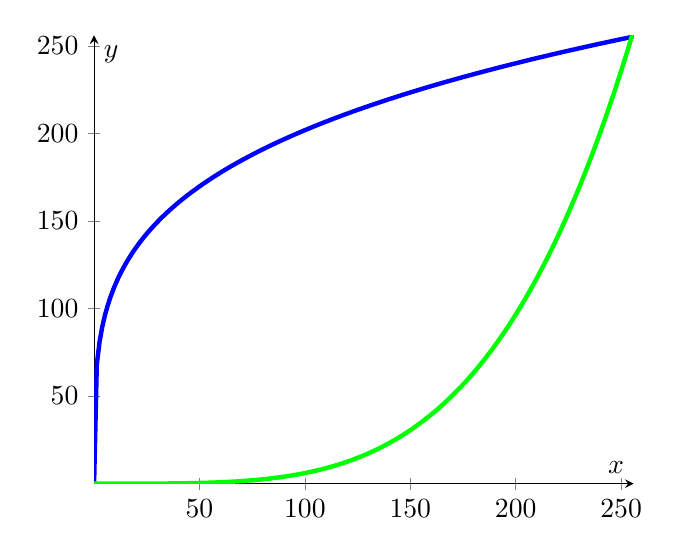
\begin{tikzpicture}[scale=1.0]
        \begin{axis}[
            axis x line=middle,
            axis y line=middle,
            ymin=0,ymax=256,ylabel=$y$,
            xmin=0,xmax=256,xlabel=$x$
            ]
        \addplot[domain=0:256, blue, ultra thick, samples=200] {255*(x/255)^0.25};
        \addplot[domain=0:256, green, ultra thick, samples=200] {255*(x/255)^4.0};
    \end{axis}
    \end{tikzpicture}
\caption{Graph of gamma function $(L-1)\left(\frac{r}{L-1}\right)^\gamma$ where $\gamma = 4$ (green) and $\gamma = \frac{1}{4}$ (blue).}
\label{fig:gamma}
\end{figure}

\begin{figure}[ht!]
    \centering
    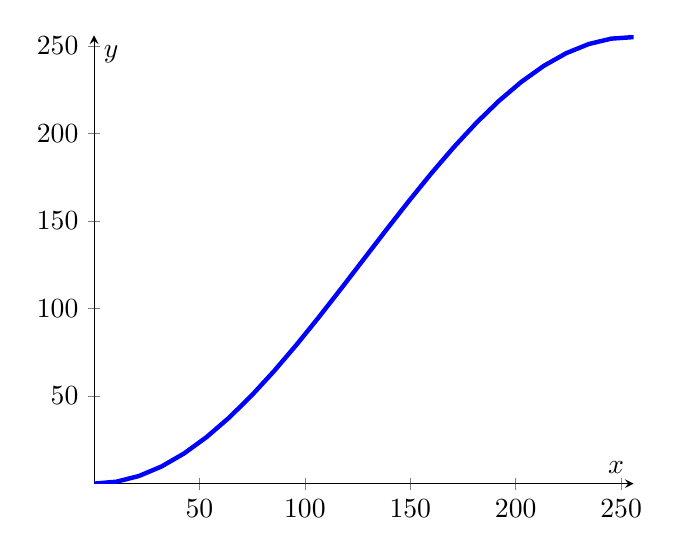
\begin{tikzpicture}[scale=1.0]
        \begin{axis}[
            axis x line=middle,
            axis y line=middle,
            ymin=0,ymax=256,ylabel=$y$,
            xmin=0,xmax=256,xlabel=$x$
            ]
        \addplot[domain=0:256, blue, ultra thick] {127.5 + 127.5*sin(deg(0.5*pi*(x - 127.5)/127.5))};
    \end{axis}
    \end{tikzpicture}
\caption{Graph of contrast enhancement $c + c\sin\left(\frac{\pi(r-c)}{2c}\right)$.}
\label{fig:contrast}
\end{figure}

For the following four examples, let $I = \begin{bmatrix}
    0 & 0 & 0\\ 255 & 255 & 0 \\ 255 & 0 & 100
\end{bmatrix}$, so $\mathbb{D} = \left[0, 2\right] \times \left[0, 2\right]$, and let $L = 2^8 = 256$ so $\mathbb{P} = \left[0, 256 - 1\right]$.

\begin{exmp}
    Identity: $T: r \mapsto r$, $J = \begin{bmatrix}
        0 & 0 & 0\\ 255 & 255 & 0 \\ 255 & 0 & 100
    \end{bmatrix}$.
\end{exmp}

\begin{exmp}
    Negative: $T: r \mapsto (L-1) - r$, $J = \begin{bmatrix}
        255 & 255 & 255 \\ 0 & 0 & 255 \\ 0 & 255 & 155
    \end{bmatrix}$.
\end{exmp}

\begin{exmp}
    Converting a grayscale image to B\&W uses a threshold function, an example of which is shown in Figure \ref{fig:threshold}. \[T: r \mapsto (L-1)H(r - t)\] where $L \geq t \geq 0$. \[J = \begin{bmatrix}
        0 & 0 & 0\\ 255 & 255 & 0 \\ 255 & 0 & 0
    \end{bmatrix}\]
\end{exmp}

\begin{exmp}
    Gamma-correction uses the gamma function, two examples of which are shown in Figure \ref{fig:gamma}. \[T: r \mapsto (L-1)\left(\frac{r}{L-1}\right)^\gamma\] where $\gamma > 0$. When $\gamma > 1$ the image is darkened, when $\gamma < 1$ the image is brightened, and when $\gamma = 1$ the image is unchanged.
\end{exmp}

\begin{exmp}
    Contrast-enhancement can be done using the function shown in Figure \ref{fig:contrast}. \[T: r \mapsto c + c\sin\left(\frac{\pi(r-c)}{2c}\right)\] where $c = \frac{L - 1}{2}$. When $\gamma > 1$ the image is darkened, when $\gamma < 1$ the image is brightened, and when $\gamma = 1$ the image is unchanged.
\end{exmp}

\subsection{Filtering and Convolutions}

\begin{defn}
    A \emph{filter mask} $w$ is a $(2k_1 + 1) \times (2k_2 + 1)$ matrix, where $k_1, k_2 \in \N$.

    \[w = \begin{bmatrix}
        w{(-k_1, -k_2)} & \cdots & w{(-k_1, 0)} & \cdots & w{(-k_1, k_2)} \\
        \vdots & \ddots & \vdots & \iddots & \vdots \\
        w{(0, -k_2)} & \cdots & w{(0, 0)} & \cdots & w{(0, k_2)} \\
        \vdots & \iddots & \vdots & \ddots & \vdots \\
        w{(k_1, -k_2)} & \cdots & w{(k_1, 0)} & \cdots & w{(k_1, k_2)} \\
    \end{bmatrix}\]
\end{defn}

\begin{exmp}
    A \emph{mean} or \emph{uniform averaging} filter uses a filter mask where
    \[w = \frac{1}{k_1k_2}\begin{bmatrix}
        1 & \cdots & 1 & \cdots & 1 \\
        \vdots & \ddots & \vdots & \iddots & \vdots \\
        1 & \cdots & 1 & \cdots & 1 \\
        \vdots & \iddots & \vdots & \ddots & \vdots \\
        1 & \cdots & 1 & \cdots & 1 \\
    \end{bmatrix}.\] Typically, averaging filters are used with a $3 \times 3$ or $5 \times 5$ mask.
\end{exmp}

\begin{exmp}
    A \emph{Gaussian} filter uses a filter mask created by sampling a Gaussian function \[g(x, y) = \frac{1}{2\pi\sigma^2}e^{-\frac{x^2+y^2}{2\sigma^2}}\] where
    \[w = \begin{bmatrix}
        g(-k_1, -k_2) & \cdots & g(-k_1, 0) & \cdots & g(-k_1, k_2) \\
        \vdots & \ddots & \vdots & \iddots & \vdots \\
        g(0, -k_2) & \cdots & g(0, 0) & \cdots & g(0, k_2) \\
        \vdots & \iddots & \vdots & \ddots & \vdots \\
        g(k_1, -k_2) & \cdots & g(k_1, 0) & \cdots & g(k_1, k_2) \\
    \end{bmatrix}.\]
\end{exmp}

\begin{defn}
    Let $I: \mathbb{D} \to \mathbb{P}$ be an image, and $w$ a filter mask. Then applying the \emph{filter} represented by $w$ to $I$ results in the image $J: \mathbb{D} \to \mathbb{D}$ defined by: \[J(i, j) = \sum_{u = -k_1}^{k_1}\sum_{v = -k_2}^{k_2}I(i + u, j + v)w(u, v).\]
\end{defn}

Notice that filters cannot be naively applied to the $k_1 + 1$ top/bottom-most rows, nor the $k_2 + 1$ left/right-most columns of $I$, since entries with indices outside the image do not exist. This problem can be solved via a variety of strategies.
\begin{itemize}
    \item One option is to zero-pad the image. For example, if $I$ is $3 \times 3$, then $I(2, 3)$ and $I(-1, 2)$ would both be $0$.
    \item Zero-padding a bright image could cause strange filter behavior near the edges, so the image could instead be padded with the average value of the entire image.
    \item Constant-padding with the average could still cause issues if parts of the image's edges differ significantly from the rest of the image, so nearest-neighbor padding can be used instead. This is where the added padding pixels have the same value as the nearest pixel from the image.
    \[\begin{array}{c c||c c c}
        3 & 3 & 3 & 7 & 2 \\
        3 & 3 & 3 & 7 & 2\\
        \hline \hline
        3 & 3 & 3 & 7 & 2 \\
        5 & 5 & 5 & 1 & 6 \\
        8 & 8 & 8 & 9 & 4 \\
    \end{array}\]
    \item Nearest-neighbor can cause issues with detecting edges that are near/coincide with the edge of the image itself. This can be solved by instead by using reflective (also symmetric)padding. The reflection of the image's outer rows/columns can help accentuate an edge if one exists, rather than suppressing it like nearest-neighbor.
    \[\begin{array}{c c||c c c}
        1 & 5 & 5 & 1 & 6 \\
        7 & 3 & 3 & 7 & 2\\
        \hline \hline
        7 & 3 & 3 & 7 & 2 \\
        1 & 5 & 5 & 1 & 6 \\
        9 & 8 & 8 & 9 & 4 \\
    \end{array}\]
    \item Periodic padding tiles the image, so accessing entries past one side will wrap around and access entries on the other side. Can be useful if images can an inherent periodicity that reflective padding doesn't take advantage of.
\end{itemize}

\begin{defn}
    Let $I: \Z^2 \to \R$ be a function representing an image $I_0: \mathbb{D} \to \mathbb{P}$ take has been extended to infinity by zero-padding. Note that $I_0$ could be another image that has been padded in some way. Let $h: \Z^2 \to \R$ be a function (called the \emph{kernel} or \emph{convolution kernel}). Then we define the \emph{convolution} of $I$ and $h$, denoted by $I * h$, as \[(I * h)(i, j) = \sum_{k=-\infty}^{\infty}\sum_{l=-\infty}^{\infty}I(i - k, j - l)(h, k, l).\] Notice the similarities to the definition of applying a filter, and the differences --- there on no bounds, and the image entries are indexed using $i - k$ and $i - l$ rather than $i + u$ and $i + v$.
\end{defn}

Filtering can be defined in terms of convolution. To apply a $(2k_1 + 1) \times (2k_2 + 1)$ filter mask $w$ to an $n \times m$ image $I$ (which may be padded), define $h(k, l) = w(-k, l)$, and extend both $h$ and $I$ to infinity by zero-padding. Then $J = I * H$.

\begin{exmp}\proofbreak
    \begin{itemize}
        \item The mean filter mask can be used as a convolution kernel to evenly blur images, smoothing them out and removing noise.
        \item The Gaussian blurring can be performed by using the Gaussian mask as a convolution kernel, resulting in less significant smoothing effects while still working to denoise the image.
    \end{itemize}
\end{exmp}

Convolution is a linear operation, however several useful filtering operations are non-linear. One example is median blurring. Similarly to how mean filtering defines $J(i, j)$ to be the mean of the neighborhood of $I(i, j)$, median blurring uses the median of the neighborhood of $I(i, j)$. This can result in superior denoising, while better preserving edges. However, it is more computationally expensive than either mean or Gaussian blurring.

\subsection{Partial Derivatives for Images}

\begin{defn}
    When $\Delta x$ is small enough, $f'(x_0)$ can be approximated using the \emph{forward difference formula}: \[f'(x_0) \approx \frac{f(x_0 + \Delta x) - f(x_0)}{\Delta x}.\]
\end{defn}

\begin{defn}
    When $\Delta x$ is small enough, $f'(x_0)$ can be approximated using the \emph{back difference formula}: \[f'(x_0) \approx \frac{f(x_0) - f(x_0 - \Delta x)}{\Delta x}.\]
\end{defn}

\begin{rmk}
    Often, for a particular function at a particular point, the forward difference formula will overestimate the derivative and the backward difference formula will underestimate it, or vice versa. Thus, the average often gives a better approximation.
\end{rmk}

\begin{defn}
    The \emph{central difference formula} (also the \emph{midpoint formula)} approximates $f'(x_0)$ for a function $f$ as the average of the forward and backward difference functions. \[f'(x_0) \approx \frac{1}{2}\left(\frac{f(x_0 + \Delta x) - f(x_0)}{\Delta x} + \frac{f(x_0) - f(x_0 - \Delta x)}{\Delta x}\right) = \frac{f(x_0 + \Delta x) - f(x_0 - \Delta x)}{2\Delta x}.\]
\end{defn}

\begin{rmk}
    We can approximate the second derivative $f''(x_0)$ of a function $f$ at point $x_0$ as \[f''(x_0) \approx \frac{f(x_0 + \Delta x) - 2f(x_0) + f(x_0 - \Delta x)}{\left(\Delta x\right)^2}\] by applying the forward difference formula to the backward difference formula or vice versa.
\end{rmk}

\begin{defn}
    These approximations of derivatives are known as \emph{finite differences}.
\end{defn}

\begin{exmp}
    Let $f: D \subseteq \R^2 \to \R$ be a function. We can use the central difference formula to approximate the first and second partial derivatives of $f(x, y)$ at $(x_0, y_0) \in \mathbb{D}$.

    \[\frac{\partial f}{\partial x}(x_0, y_0) \approx \frac{f(x_0 + \Delta x, y_0) - f(x_0 - \Delta x, y_0)}{2\Delta x}.\]

    \[\frac{\partial f}{\partial y}(x_0, y_0) \approx \frac{f(x_0, y_0  + \Delta y) - f(x_0, y_0 - \Delta y)}{2\Delta y}.\]

    \[\frac{\partial^2 f}{\partial x^2}(x_0, y_0) \approx \frac{f(x_0 + \Delta x, y_0) - 2f(x_0, y_0) + f(x_0 - \Delta x, y_0)}{\left(\Delta x\right)^2}.\]
\end{exmp}

\begin{rmk}
    To apply these formulas to images, we have $x_0 = j$, $y_0 = i$, and $\Delta x = \Delta j = 1$, $\Delta y = \Delta i = 1$.
\end{rmk}

\begin{exmp}
    Let $I: \mathbb{D} \to \mathbb{P}$ be an image. Then the following are approximations of the derivatives of $I$ at $(i, j) \in \mathbb{D}$:
    \[\frac{\partial^2I}{\partial y^2}(i, j) \approx \frac{I(i + 1, j) - 2I(i, j) + I(i - 1, j)}{1^2},\]
    \[\frac{\partial I}{\partial y}(i, j) \approx \frac{I(i + 1, j) - I(i - 1, j)}{2},\]
    \[\frac{\partial I}{\partial x}(i, j) \approx \frac{I(i, j + 1) - I(i, j - 1)}{2},\]
\end{exmp}

Since $\frac{\partial I}{\partial y}(i, j) \approx \frac{I(i + 1, j) - I(i - 1, j)}{2} = \frac{1}{2}I(i + 1, j) - \frac{1}{2}I(i - 1, j)$ for some image $I: \mathbb{D} \to \mathbb{P}$, we can find $\frac{\partial I}{\partial y}$ for every $(i, j) \in \mathbb{D}$ by filtering $I$ with the filter mask \[w_y = \begin{bmatrix}
    0 & -1/2 & 0 \\
    0 & 0 & 0 \\
    0 & 1/2 & 0 \\
\end{bmatrix}.\] This is equivalent to the convolution $I * h_y$, where \[h_y = \begin{bmatrix}
    0 & 1/2 & 0 \\
    0 & 0 & 0 \\
    0 & -1/2 & 0 \\
\end{bmatrix}.\]

In practice, the Prewitt or Sobel filters are much more frequently used.

Prewitt filter: \[w_y^P = \frac{1}{6}\begin{bmatrix}
    -1 & -1 & 1 \\
    0 & 0 & 0 \\
    1 & 1 & 1 \\
\end{bmatrix}\]

Sobel filter: \[w_y^S = \frac{1}{8}\begin{bmatrix}
    -1 & -2 & -1 \\
    0 & 0 & 0 \\
    1 & 2 & 1 \\
\end{bmatrix}\]

The Prewitt filter uses the average of three adjacent first derivatives in order to smooth out noise, and the Sobel filter does the same, but with a weighted average.

\subsection{Laplacian for Images}

\begin{defn}
    Let $f: \R^n \to \R$ be a twice-differentiable function. The \emph{Laplacian} of $f$ is the sum of all unmixed second order partial derivatives.

    \[\nabla^2f(x_1, \ldots, x_n) = \sum_{i=1}^n \frac{\partial^2f}{\partial x_i^2}(x_1, \ldots, x_d)\]
\end{defn}

\begin{exmp}
    Let $f: \R^2 \to \R$. Then at some $(x_0, y_0) \in \R^2$, \[\nabla^2 f(x_0, y_0) = \frac{\partial^2f}{\partial x^2}(x_0, y_0) + \frac{\partial^2f}{\partial y^2}(x_0, y_0).\]
\end{exmp}

\begin{defn}
    Let $I: \mathbb{D} \to \mathbb{P}$ be an image. Then its \emph{Laplacian} is defined by \[\nabla^2I(i, j) = (I * h_{xx})(i, j) + (I * h_{xx})(i, j),\] where $h_xx$ and $h_yy$ are kernels for the approximation of the images second derivatives.
\end{defn}

Since convolution distributes over addition of kernels, \[(I * h_{xx})(i, j) + (I * h_{xx})(i, j) = \left(I * (h_{xx} + h_{xx}\right)(i, j).\] Let $h_L = h_{xx} + h_{yy}$, then
\[h_L = \begin{bmatrix}
    0 & 1 & 0 \\ 1 & -4 & 1 \\ 0 & 1 & 1
\end{bmatrix}.\]

The following kernels are more frequently used to practice, which they use a weighted average of adjacent values as with the Prewitt and Sobel filters:

\[h_{L_8} = \begin{bmatrix}
    1 & 1 & 1 \\ 1 & -8 & 1 \\ 1 & 1 & 1
\end{bmatrix}\]

\[h_{L_12} = \begin{bmatrix}
    1 & 2 & 1 \\ 2 & -12 & 2 \\ 1 & 2 & 1
\end{bmatrix}\]

The Laplacian of an image can be used to sharpen the image. For example, consider the logistic function, its first derivative, and its Laplacian, which are shown in Figure \ref{fig:laplacian} as the blue, green, and red graphs respectively.

\[f(x) = \frac{e^x}{e^x + 1}\]
\[\nabla{f} = \frac{e^x}{(e^x + 1)^2}\]
\[\nabla^2f(x) = \frac{e^x - e^{3x}}{(e^x + 1)^4}\]

\begin{figure}[ht!]
    \centering
    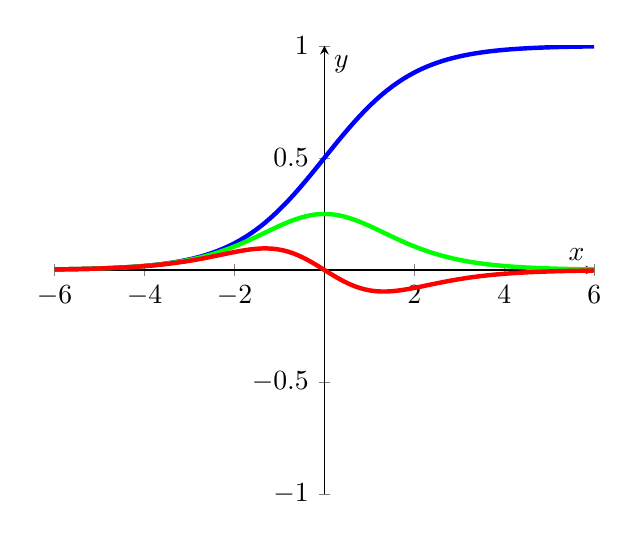
\begin{tikzpicture}[scale=1.0]
        \begin{axis}[
            axis x line=middle,
            axis y line=middle,
            ymin=-1,ymax=1,ylabel=$y$,
            xmin=-6,xmax=6,xlabel=$x$
            ]
        \addplot[domain=-6:6, blue, ultra thick, samples=100] {e^x/(e^x+1)};
        \addplot[domain=-6:6, green, ultra thick, samples=100] {e^x/(e^x+1)^2};
        \addplot[domain=-6:6, red, ultra thick, samples=100] {(e^x-e^(3*x))/(e^x+1)^4};
    \end{axis}
    \end{tikzpicture}
\caption{Graph of the logistic function, its first derivative, and its Laplacian.}
\label{fig:laplacian}
\end{figure}

Now consider the function $g(x) = f(x) - k\nabla^2f(x)$ for some positive real constant $k$. $g(x)$ for the logistic function with $k=2$ is shown in red in comparison to the logistic function in blue in Figure \ref{fig:laplacian-sharpening}. This technique will sharpen any twice-differentiable function, as it will essentially ``pull-down'' concave-down parts of the function, and ``push-up'' concave-up parts of the function. The effect of this is to accentuate corners and make regions are inflection points steeper.

\begin{figure}[ht!]
    \centering
    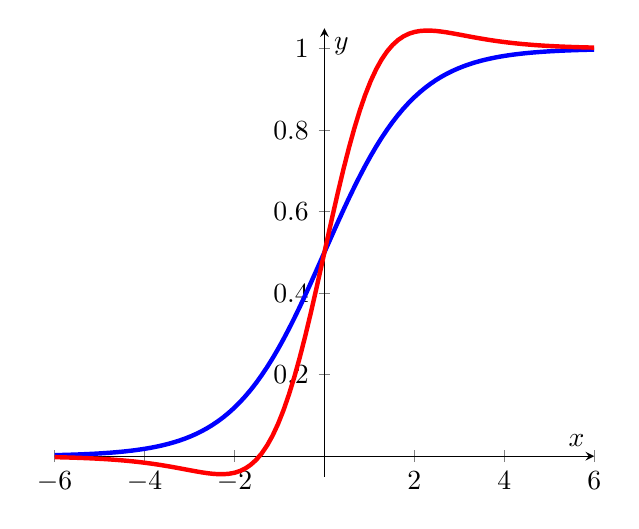
\begin{tikzpicture}[scale=1.0]
        \begin{axis}[
            axis x line=middle,
            axis y line=middle,
            ymin=-0.05,ymax=1.05,ylabel=$y$,
            xmin=-6,xmax=6,xlabel=$x$
            ]
        \addplot[domain=-6:6, blue, ultra thick, samples=100] {e^x/(e^x+1)};
        \addplot[domain=-6:6, red, ultra thick, samples=100] {e^x/(e^x+1) - 2*((e^x-e^(3*x))/(e^x+1)^4)};
    \end{axis}
    \end{tikzpicture}
\caption{Graph of $f(x) - k\nabla^2f(x)$, where $k=2$.}
\label{fig:laplacian-sharpening}
\end{figure}

We can apply this technique to an entire image. Let $I: \mathbb{D} \to \mathbb{P}$ be an image, then define $J$ by \[J(i, j) = I(i, j) - k\nabla^2I(i, j),\] for all $(i, j) \in \mathbb{D}$ and some real $k > 0$.

\subsection{Image Processing on Graphs}

We can apply graph theory and signal processing to image processing by modelling image data as graph signals. We will first define graphs and graph signals, and then explore how they can be applied to image processing.

\begin{defn}
    An \emph{undirected graph} is a $2$-tuple $\mathcal{G} = (\mathcal{V}, \mathcal{E})$, where $\mathcal{V}$ is a set of vertices, and $\mathcal{E}$ is a set of unordered pairs (two-sets) of vertices, called edges.
\end{defn}

\begin{defn}
    The \emph{adjacency matrix} $\bm{A}$ of a graph $\mathcal{G} = (\mathcal{V}, \mathcal{E})$ is a square $|\mathcal{V}| \times |\mathcal{V}|$ matrix where $\bm{A}_{i, j}$ is $1$ if there is an edge from $\mathcal{V}_i$ to $\mathcal{V}_j$, and $0$ otherwise.
\end{defn}

\begin{exmp}
    Let $\mathcal{V} = \{1, 2, 3, 4\}$, let $\mathcal{E} = \{\{1, 2\}, \{2, 3\}, \{3, 4\}, \{4, 1\}\}$. Then $\mathcal{G} = (\mathcal{V}, \mathcal{E})$ is the graph shown in Figure \ref{fig:example-graph}. The adjacency matrix of $\mathcal{G}$ is
    \[\bm{A} = \begin{bmatrix}
        0 & 1 & 0 & 1 \\
        1 & 0 & 1 & 0 \\
        0 & 1 & 0 & 1 \\
        1 & 0 & 1 & 0
    \end{bmatrix}.\]
\end{exmp}

\begin{figure}[ht!]
    \centering
    \begin{tikzpicture}
        \begin{scope}[every node/.style={circle,thick,draw,fill=cyan}]
            \node (1) at (0,0) {1};
            \node (2) at (2,0) {2};
            \node (3) at (2,2) {3};
            \node (4) at (0,2) {4};
        \end{scope}

        \begin{scope}[>={Stealth[black]},
            every node/.style={fill=white,circle},
            every edge/.style={draw=black,very thick}]
            \path [<->] (1) edge (2);
            \path [<->] (2) edge (3);
            \path [<->] (3) edge (4);
            \path [<->] (4) edge (1);
        \end{scope}
    \end{tikzpicture}
\caption{Example graph.}
\label{fig:example-graph}
\end{figure}

\begin{defn}
    A \emph{weighted, undirected graph} is a $3$-tuple $\mathcal{G} = (\mathcal{V}, \mathcal{E}, \bm{W})$, where $\mathcal{V}$ is a set of vertices, $\mathcal{E}$ is a set of unordered pairs (two-sets) of vertices, called edges, and $\bm{W}$ is a square $|\mathcal{V}| \times |\mathcal{V}|$ real matrix of weights. The weight between edges $i, j \in \mathcal{V}$ is $\bm{W}_{i, j}$. Note that since $\mathcal{G}$ is undirected, $\bm{W}_{i,j} = \bm{W}_{j, i}$ for all $i, j \in \mathcal{V}$, and additionally we require $\bm{W}_{i, j} \geq 0$.
\end{defn}

\begin{exmp}
    Let $\mathcal{V} = \{1, 2, 3, 4\}$, let $\mathcal{E} = \{\{1, 2\}, \{2, 3\}, \{3, 4\}, \{4, 1\}\}$, and let
    \[\bm{W} = \begin{bmatrix}
        0 & 1/2 & 0 & 1/5 \\
        1/2 & 0 & 1/3 & 0 \\
        0 & 1/3 & 0 & 1/4 \\
        1/5 & 0 & 1/4 & 0
    \end{bmatrix}.\] Then $\mathcal{G} = (\mathcal{V}, \mathcal{E}, \bm{W})$ is the graph shown in Figure \ref{fig:example-weighted-graph}.
\end{exmp}

\begin{figure}[ht!]
    \centering
    \begin{tikzpicture}
        \begin{scope}[every node/.style={circle,thick,draw,fill=cyan}]
            \node (1) at (0,0) {1};
            \node (2) at (4,0) {2};
            \node (3) at (4,4) {3};
            \node (4) at (0,4) {4};
        \end{scope}

        \begin{scope}[>={Stealth[black]},
                    every node/.style={fill=white,circle},
                    every edge/.style={draw=black,very thick}]
            \path [<->] (1) edge node {$1/2$} (2);
            \path [<->] (2) edge node {$1/3$} (3);
            \path [<->] (3) edge node {$1/4$} (4);
            \path [<->] (4) edge node {$1/5$} (1);
        \end{scope}
    \end{tikzpicture}
\caption{Example weighted graph.}
\label{fig:example-weighted-graph}
\end{figure}

\begin{defn}
    Let $\mathcal{G} = (\mathcal{V}, \mathcal{E})$ be a graph. Then a \emph{graph signal} $f: \mathcal{V} \to \R$ is simply a function which assigns a real value to each vertex. The image of $f$ can be represented as a vector $v$ where the $i$-th entry is $f(i)$ --- the value associated with the $i$-th vertex.
\end{defn}

\begin{defn}
    The \emph{degree} of a vertex $v$ is the number of edges containing $v$.
\end{defn}

\begin{defn}
    The \emph{degree matrix} $\bm{D}$ of an unweighted graph $\mathcal{G} = (\mathcal{V}, \mathcal{E})$ is a square $|V| \times |V|$ matrix that is all zero, except for the diagonal entries. The $n$-th diagonal entry is the degree of the $n$-th vertex of $\mathcal{G}$. It follows that $\bm{D}$ is related to the adjacency matrix $\bm{A}$ by \[\bm{D}_{n,n} = \sum_{i=0}^{|V|}\bm{A}_{n,i}.\]
\end{defn}

\begin{defn}
    The concept of a \emph{degree matrix} $\bm{D}$ can be extended to a weighted graph $\mathcal{G} = (\mathcal{V}, \mathcal{E}, \bm{W})$. It is defined by \[\bm{D}_{n,n} = \sum_{i=0}^{|V|}\bm{W}_{n,i}.\]
\end{defn}

\begin{defn}
    The \emph{graph Laplacian} $\bm{L}$ of a weighted graph $\mathcal{G} = (\mathcal{V}, \mathcal{E}, \bm{W})$ is $L = D - W$.
\end{defn}

An image $I: \mathbb{D} \to \mathbb{P}$ can be represented as a graph signal. First, assign each pixel to a vertex, and then create an edge between every pixel's horizontal, vertical, and diagonal neighbors. Then the image can be encoded as the function $f: \mathbb{D} \to \mathbb{P}$ that assigns the value of each pixel to the corresponding vertex.

\section{Shapes}

\subsection{Mathematically Describing Shapes}

\begin{defn} (Due to Wikipedia)
    A \emph{shape} is the form of an object or its boundary, as opposed to other properties of the shape, such as its color, texture, material, position, or orientation.
\end{defn}

\begin{defn} (Due to David G. Kendall)
    A \emph{shape} is the geometrical information that remains when the position, scale, and rotation  of an object are ignored.
\end{defn}

\begin{defn}
    Consider a parameter space $M$. A \emph{parameterized curve} is a continuous mapping $c: M \to \R^d$. $M$ is usually an interval:
    \begin{enumerate}
        \item $M = [a, b]$, e.g. $M = [0, 1]$ for open curves,
        \item $M = S^1$ (the unit circle) for closed curves.
    \end{enumerate}
\end{defn}

\begin{exmp}
    Let $M = [0, 1]$ and $d = 1$. Then \emph{one-dimensional} curves are mappings of the form $c: M \to \R$ where $c(t) = f(t)$ for some function $f$.
    \begin{itemize}
        \item $c(t) = 2t - 1$ gives a particular line.
        \item $c(t) = (t - \frac{1}{2})^2$ describes a particular parabola.
    \end{itemize}
\end{exmp}

\begin{exmp}
    Let $M = [0, 1]$ and $d = 2$. Then \emph{two-dimensional} curves are mappings of the form $c: M \to \R^2$ where $c(t) = (x(t), y(t))$ for some functions $x, y$.
    \begin{itemize}
        \item $c(t) = (\cos(2\pi{t}), \sin(2\pi{t}))$ describes the unit circle.
    \end{itemize}
\end{exmp}

\begin{rmk}
    Shapes can be described as parametric curves/surfaces.
\end{rmk}

\begin{exmp}
    If we want to parameterize a triangle on $M = [0, 1]$, we can use piecewise functions. For example,
    \[c(t) = \left\{
        \begin{array}{ll}
          (t, 0) & : t \in [0, 1/3)\\
          (1/3, t - 1/3) & : t \in [1/3, 2/3)\\
          (1 - t, 1 - t) & : t \in [2/3, 1]\\
        \end{array}
      \right.
    \]
\end{exmp}

\begin{defn}
    From here, a \emph{shape} is a two-dimensional parametric curve $c: M \to \R^2$ on some interval $M$, which is in differentiable continuity class $C^1$ and $c'(t) \neq 0$ for all $t \in M$.
\end{defn}

\begin{defn}
    An \emph{immersion} between $\R^n$ and $\R^m$ is a differentiable function $f: \R^n \to \R^m$ whose derivative at any point $p \in \R^n$ is linear map that is everywhere injective.
\end{defn}

\begin{rmk}
    An immersion between $\R$ and $\R^2$ on some domain $M \subseteq \R$ is then a differentiable function \[c: M \to \R^2\] \[c(t) \mapsto (x(t), y(t)),\] where $\norm{c'(t)} \neq 0$ for all $t \in M$. It follows that shapes are immersions between $\R$ and $\R^2$.
\end{rmk}

\begin{defn}
    Let $c: M \to \R^2$ be a shape, with $c(t) = (x(t), y(t))$. Then the \emph{tangent} vector of $c$ at $t$, denoted by $T_c(t)$, is the unique unit vector in the direction $c'(t)$. The \emph{normal} vector of $c$ at $t$, denoted by $N_c(t)$, is the unique vector which extends $T_c(t)$ to a positively oriented orthonormal basis for $\R^n$.
\end{defn}

\begin{prop}
    The tangent vector of $c$ at $t$ is given by \[T_c(t) = \frac{c'(t)}{\norm{c'(t)}} = \frac{(x'(t), y'(t))}{\sqrt{(x'(t))^2 + (y'(t))^2}}.\]
\end{prop}

\begin{proof}
    It is clear that \[\norm{T_c(t)} = \frac{\norm{(x'(t), y'(t))}}{\sqrt{(x'(t))^2 + (y'(t))^2}} = \frac{\sqrt{(x'(t))^2 + (y'(t))^2}}{\sqrt{(x'(t))^2 + (y'(t))^2}} = 1,\] and that since $T_c(t) = \frac{1}{\sqrt{(x'(t))^2 + (y'(t))^2}}c'(t)$, it must be parallel to $c'(t)$, so it is the tangent vector.
\end{proof}

\begin{prop}
    The normal vector of $c$ at $t$ is given by \[N_c(t) = \frac{(-y'(t), x'(t))}{\sqrt{(x'(t))^2 + (y'(t))^2}}.\]
\end{prop}

\begin{proof}
    It is clear that $\norm{N_c(t)} = \norm{T_c(t)} = 1$, so $N_c(t)$ is a unit vector. Since \[\left\langle T_c(t), N_c(t) \right\rangle = \frac{1}{(x'(t))^2 + (y'(t))^2}\left(x'(t)(-y'(t)) + y'(t)x'(t)\right) = 0,\] $N_c(t)$ is orthogonal to $T_c(t)$, and so extends $T_c(t)$ to an orthonormal basis for $\R^2$. Furthermore, since \[\det\begin{pmatrix}
        T_c(t) & N_c(t)
    \end{pmatrix} = \frac{1}{\norm{c'(t)}^2}\begin{vmatrix}
        x'(t) & -y'(t) \\ y'(t) & x'(t)
    \end{vmatrix} = \frac{x'(t)^2 + y'(t)^2}{x'(t)^2 + y'(t)^2} = 1,\] the ordered orthonormal basis $\left\langle T_c(t), N_c(t) \right\rangle$ is positively oriented.
\end{proof}

\subsection{Properties of Shapes}

In this section, we will extend the definition of several useful properties of circles to arbitrary shapes.

\begin{defn}
    The \emph{diameter} of a shape $c$ is the largest of the maximum width and maximum height of the shape.
\end{defn}

\begin{defn}
    The \emph{arc length} of a shape $c: M \to \R^2$, denoted by $L_c$, is the extension of circumference, and is given by \[L_c = \int_M\norm{c'(t)}dt = \int_M{\sqrt{x'(t)^2 + y'(t)^2}}dt.\] The expression ${\sqrt{x'(t)^2 + y'(t)^2}}dt$ is sometimes called the arc length measure, denoted $ds$, giving $L_c = \int_M ds$.
\end{defn}

\begin{defn}
    The \emph{centroid} of a shape $c: M \to \R^2$ is the point $(\bar{x}, \bar{y})$, where \[\bar{x} = \int_M x(t)\frac{ds}{L_c},\] \[\bar{y} = \int_M y(t)\frac{ds}{L_c}.\]
\end{defn}

\begin{defn}
    The \emph{convex hull} of a shape $c$ is the minimum convex shape which completely encloses $c$.
\end{defn}

\begin{defn}
    The \emph{discretization} of a curve $c: M \to \R^2$ where into $N$ pieces is the set $\{c(t_n) : 0 \leq n < N\}$, where $M$ is divided into $N$ intervals and $t_n$ denotes the zero-indexed $n$th interval. This can also be represented as the $N \times 2$ matrix
    \[\begin{bmatrix}
        c(t_0) \\ \vdots \\ c(t_{N-1})
    \end{bmatrix} = \begin{bmatrix}
        x_0 & y_0 \\ \vdots & \vdots \\ x_{N-1} & y_{N-1}
    \end{bmatrix}.\]
\end{defn}

To compute the derivative of a discretized curve $c: M \to \R^2$ at some $t_k \in M$, we can use finite differences, so \[c'(t_k) \approx \frac{c(t_{k+1})- c(t_{k-1})}{2} = \left(\frac{x(t_{k+1}) - x(t_{k-1})}{2}, \frac{y(t_{k+1}) - y(t_{k-1})}{2}\right).\]

\subsection{Shape Spaces}

\begin{defn} Metric Space

    Let $S$ be a set. A \emph{distance} defined on $S$ is a function $d: S \times S \to \R$ such that
    \begin{enumerate}
        \item $d(x, y) \geq 0 \,\forall x, y \in S$,
        \item $d(x, y) = 0 \iff x = y$,
        \item $d(x, y) = d(y, x) \,\forall x, y \in S$,
        \item $d(x, y) \leq d(x, z) + d(z, y) \,\forall x, y, z \in S$.
    \end{enumerate}
    The object $(S, d)$ is a \emph{metric space}.
\end{defn}

\begin{exmp}\proofbreak
    \begin{itemize}
        \item $S = \R$, and $d(x, y) = \abs{x - y}$,
        \item $S = \R^2$, and $d(x, y) = \norm{x - y}_2 = \sqrt{(x_1-y_1)^2+(x_2-y_2)^2}$.
    \end{itemize}
\end{exmp}

\begin{defn}
    Let $S = \R^d$. Then the $L_p$ norm is a distance function $d: S \times S \to \R$ where \[d(x - y) = \norm{x - y}_p = \left(\sum_{i=1}^d(x_i - y_i)^p\right)^{1/p},\] and together with $S$ forms a metric space.
\end{defn}

We can construct a metric space on the space of parameterized curves. Let $S$ be the set of immersions between $M \subset \R$ and $\R^2$.
\[S = \left\{c \in C^1(M, \R^2) \compbar \norm{c'(t)} \neq 0 \right\}\]

We define the \emph{square root velocity transform} $Q$
\[Q: S \to L^2(M, \R^2)\]
\[Q: c(t) \mapsto \left\{
    \begin{array}{ll}
        \frac{c'(t)}{\sqrt{\norm{c'(t)}}} & : c'(t) \neq 0\\
        0 & : c'(t) = 0\\
    \end{array}
  \right.
\]

$L^2$ means square integrable, meaning $f: M \to \R^2$ if $\int_M \norm{f(t)}^2dt < \infty$. For any $q_1, q_2 \in L_2(M, \R^2)$, we define the distance function
\[d(q_1, q_2) = \sqrt{\langle q_1 - q_2, q_1 - q_2\rangle}\] where
\[\langle q_1 - q_2, q_1 - q_2 \rangle = \int_M\norm{q_1 - q_2}^2dt.\]

\begin{exmp}
    Consider the curve $s = \{\cos(t), \sin(t)\}$ on $M = [0, 2\pi]$. Then since
    \[Q(s) = \left(-\sin(t), \cos(t)\right),\] and
    \[\langle Q(s) - Q(s), Q(s) - Q(s) \rangle = \int_0^{2\pi} 0dt,\] we have
    \[d(s, s) = 0.\]
\end{exmp}

\begin{exmp}
    Consider the curves $s_1 = \{\cos(t), \sin(t)\}$, $s_2 = \{\cos(-t), \sin(-t)\}$ on $M = [0, 2\pi]$. Then since
    \[Q(s_1) = \left(-\sin(t), \cos(t)\right), Q(s_2) = \left(\sin(-t), -\cos(-t)\right),\] so
    \[Q(s_1) - Q(s_2) = 2\cos(t)\] and since
    \[\langle Q(s_1) - Q(s_2), Q(s_1) - Q(s_2) \rangle = \int_0^{2\pi}{4\cos^2(t)}dt = 4\pi,\] so we have
    \[d(s_1, s_2) = \sqrt{4\pi}.\]
\end{exmp}

Now consider the equivalence relation where for $s_1, s_2 \in S$, $s_1 \sim s_2$ means $s_1 = s_2 \circ \gamma$ for some absolutely continuous re-parameterization function $\gamma$. Then, form the quotient set $Q(S)/\sim$. We finally define the metric on $S$ to be
\[d(s_1, s_2) = \inf_{w_1\in[Q(s_1)],w_2\in[Q(s_2)]}d(w_1,w_2).\]

\begin{exmp}
    Let $s_1 = \{\cos(t), \sin(t)\}$, $s_2 = \{\cos(-t), \sin(-t)\}$ on $M = [0, 2\pi]$, and let $\gamma(t) =  -t$. Then since $s_2 = s_1 \circ \gamma$, we have $s_2 \in [s_1]$. As $d(s_1, s_1) = 0$, and $d(s, s) \geq 0$, it follows that the infimum of $d(w_1, w_2)$ where $w_1 \in [Q(s_1)]$ and $w_2 \in [Q(s_2)]$ must be zero.
\end{exmp}

``Precise Matching of PL Curves in $\R^N$ In The Square Root Velocity Framework'' by Sayani Lahiri, Daniel Robinson, and Eric Klassen \url{https://arxiv.org/pdf/1501.00577.pdf} gives more details on the theoretical basis for this approach, and an exact algorithm to solve this distance function.

``Fast Dynamic Programming for Elastic Registration of Curves'' by Javier Bernal, G\"unay Do\u{g}an, and Charles R. Hagwood \url{https://math.nist.gov/~JBernal/adapt_dp.pdf} describes a dynamic programming approach to computing the distance function.

For a relaxed, estimation solution to computing this distance function, see ``An inexact matching approach for the comparison of plane curves with general elastic metric'' by Yashil Sukurdeep, Martin Bauer, and Nicolas Charon \url{https://arxiv.org/pdf/2001.02858.pdf}.

\subsection{Shape Clustering}

Given $N$ shapes $\{c_1, c_2, \ldots, c_N\}$, let $d_{i,j}$ be $d(c_i, c_j)$ --- the distance between shapes $c_i$ and $c_j$ given by the square root velocity transform metric described above. By projecting this shapes into $\R^2$ or $\R^3$ in such as way as to preserve the pair-wise distances between the shapes, we can then apply standard clustering algorithms for points to identify clusters of shapes.

Let $\hat{x}_1, \ldots, \hat{x}_N \in \R^d$ be the projected points. Note that $d$ is typically chosen to be $2$ or $3$, so that the projected points can be visualized effectively. We can perform the desired projection by solving the optimization problem
\[\min_{\hat{x}_1, \ldots, \hat{x}_N \in \R^d}\sum_{i, j}\left(\norm{\hat{x}_i - \hat{x}_j}_2 - d_{i, j}\right)^2.\]

Form the matrix
\[D = \begin{bmatrix}
    d_{1, 1} & \cdots & d_{1, N} \\
    \vdots & \ddots & \vdots \\
    d_{N, 1} & \cdots & d_{N, N}
\end{bmatrix},\] and let $D^{(2)}$ be the element-wise square of $D$.

Let $I_N$ be the $N \times N$ identity matrix, and $O_N$ be the $N \times N$ matrix where each element is $1$. Let $J = I_N - \frac{1}{N}O_N$.

Now consider the matrix $B = \frac{-1}{2}JD^{(2)}J$. Computing this matrix is known as performing ``double-centering'', where each multiplication by $J$ is ``centering''. Let $\lambda_1, \ldots, \lambda_d$ be the $d$ largest eigenvalues of $B$, and $v_1, \ldots, v_d$ the corresponding eigenvectors. Form the matrices
\[V_d = \begin{bmatrix}
    v_1 & \cdots & v_d
\end{bmatrix},\]
\[\Lambda_d^{1/2} = \begin{bmatrix}
    \lambda_1^{1/2} & 0 & \cdots & 0 \\
    0 & \lambda_2^{1/2} & \cdots & 0 \\
    \vdots & \vdots & \ddots & \vdots \\
    0 & 0 & \cdots & 0 \\
\end{bmatrix},\] which are $N \times d$ and $d \times d$ matrices respectively.

Finally, form the $N \times d$ matrix $\hat{X} = V_d\Lambda_d^{1/2}$. Then the $i$-th row of $\hat{X}$ is $\hat{x}_i \in \R^d$. Since these are points in $\R^d$ where $\norm{\hat{x}_i - \hat{x}_j}_2 \approx d_{i, j}$, we can now apply standard clustering algorithms, such as $k$-means, to find cluster among the points. It is important to pick a good target dimension for the projection, as using very small $d$ can result in underfitting, and high $d$ can result in overfitting. Using $d=3$ is the highest possible dimension that can still be visually inspected easily, and so is often a good choice.

This process is known as ``Classical Multidimensional Scaling'', or CMDS, and is part of a larger family of projection algorithms known as MDS. Since forming the matrix $D$ did not depend at all on the square root velocity transform distance metric, this process is much more widely applicable to clustering data.
